\subsection{Resumen}

El uso de la cache es distinto para ambos compiladores: Usando programas para ver el contenido y el uso del cache (como por ejemplo valgrind) procesaremos varias imágenes, de distintos tamaños y no cuadradas, para corroborar que de acuedo al compilador, el uso de la cache varía. Primero vamos a comparar ambos sin optimización alguna. Luego vamos a repetir los experimentos activando las optimizaciones para ambos casos. \\


\subsection{Experimentaciones de caché sin optimización}

Veremos a continuacion si el uso de la cache por ambos compiladores es igual, similar o completamente diferente. Nosotros esperamos ver que sea diferente. Para esto realizaremos varias pasadas con los filtros implementados en c a diferentes imagenes utilizando dos compiladores diferentes, ICC y GCC sin la opción para optimizar. \\

Utilizaremos el valgrind, el cual nos muestra los \textit{misses} y las prediciones de saltos fallidos, dependiendo de esos resultados podremos concluir si el uso de la cache es igual de eficiente o si varía .\\

Primero veremos como es el comportamiento con el filtro blur. Por cuestiones referentes al tiempo vamos a utilizar un radio chico ya que a medida que aumenta el radio, el emulador tiene un costo temporal demasiado elevado.Usamos en este caso radio 10 y lo que va a ir variando es el tamaño de la imagen. Si hay diferencias en el uso de la cache con radios chicos, con radios mas grandes esta diferencia se va a mantener o incluso aumentar, por eso consideramos que fijar el radio no perjudica nuestro experimento. \\

\subsection{Datos obtenidos:}

\begin{figure}[H]
\begin{center}
%\minipage{0.8\textwidth}
  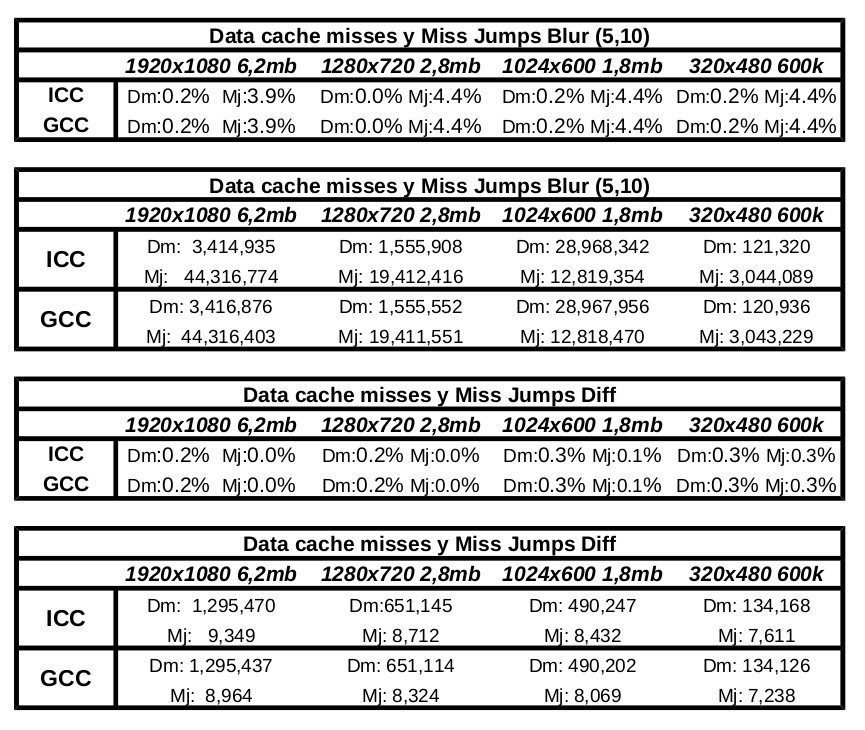
\includegraphics[width=\linewidth]{cachecompiladores/tabla.png}
%\endminipage
\end{center}
\end{figure}

\subsection{Conclusion}

Luego de obtener los resultados y analizarlos observamos que si bien los valores de misses y miss jumps son muy parecidos , no son lo suficientemente parecidos como para concluir que el uso de la cache que hacen ambos compiladores es el mismo. Esto lo deducimos porque vimos que cuando corrimos varias veces el mismo filtro a la misma imagen utilizando siempre solo un compilador, al ver los resultados (los miss cache), estos varian entre si en muy poco (+- diez ), pero si compramos los resultados de misses obtenidos utilizando compiladores diferentes estas variaciones son suficientemente grandes como para ver que definitivamente no hacen lo mismo. \\

Por otro lado si miramos los porcentajes, se observa que ambos tienen exatamente los mismos, por eso concluimos que no eran necesarios graficos, pues los valores son exactamente iguales, para cualquiera de los dos filtros, en cualquier situacion. Finalmente podemos concluir que en realidad los compiladores manejan la cache de maneras distintas al menos sin las optimizaciones activas. Como un detalle, se puede ver que ICC tiende a tener mas misses y miss jumps que GCC. Antes habiamos visto que ICC es un poco mas rápido que GCC. Aquí podemos confirmar que eso no se debe a un mejor uso de la caché.


\subsection{Experimentaciónes de la caché con optimizaciones activas}

Para esta faceta del experimento vamos a activar la opción de optimización \textit{-O3}para ambos compiladores y vamos a ver como esto influye en el manejo de la memória caché. Lo que esperamos ver en los experimentos realizados en esta sección es un manejo diferenciado de la memoría por ambos compiladores.\\

ACÁ HAY QUE HACER VARIOS EXPERIMENTOS CON IMÁGENES USANDO LA OPCIÓN -O3 Y VER COMO ESO AFECTA A LA CACHÉ. SI EL MANEJO ES DISTINTO. GANAMOS Y CONFIRMAMOS NUESTRA HIPOTESIS. POR EL CONTRARIO SI VEMOS QUE LA CACHE SE COMPORTA IGUAL PODEMOS REFUTAR NUESTRA HIPOTESIS.

\subsection{Conclusiones:}
Con los experimentos detallados anteriormente podemos llegar a la conclusión de que los compiladores ICC y GCC con la opción de optimización \textit{-O3} manejan la caché de manera distinta/similar y esto nos ayuda a corroborar/refutar nuestra hipótesis.
